% Metódy inžinierskej práce

\documentclass[10pt,twoside,english,a4paper]{article}

\usepackage[english]{babel}
%\usepackage[T1]{fontenc}
\usepackage[IL2]{fontenc} % lepšia sadzba písmena Ľ než v T1
\usepackage[utf8]{inputenc}
\usepackage{graphicx}
\usepackage{url} % príkaz \url na formátovanie URL
\usepackage{hyperref} % odkazy v texte budú aktívne (pri niektorých triedach dokumentov spôsobuje posun textu)
\usepackage{pdfpages}
\usepackage{cite}
%\usepackage{times}

\pagestyle{headings}

\title{Role-playing games, their development and interactive storytelling\thanks{Semestrálny projekt v predmete Metódy inžinierskej práce, ak. rok 2022/23, vedenie: Meno Priezvisko}} % meno a priezvisko vyučujúceho na cvičeniach

\author{Gabriel Ábrahám\\[2pt]
	{\small Slovenská technická univerzita v Bratislave}\\
	{\small Fakulta informatiky a informačných technológií}\\
	{\small \texttt{xabraham@stuba.sk}}
	}

\date{\small 11.10.2022} 



\begin{document}

\maketitle

\begin{abstract}
The development of tabletop role-playing games to modern 
computer role-playing games was enormous, introducing a new and 
different experience from books for getting immersed in a story. This 
work introduces RPGs, and their genres in-depth and presents their 
elements in some examples, elaborating on their 
history/development from physical tabletop roleplaying to software-based RPGs with many genres including the adaptation which is the 
closest to the tabletop version. Also introduces their interactive 
storytelling, which is one of their most famous elements, and why it 
could also serve as an alternative for classic reading.

Keywords – role-playing games, interactive storytelling, video games
\end{abstract}


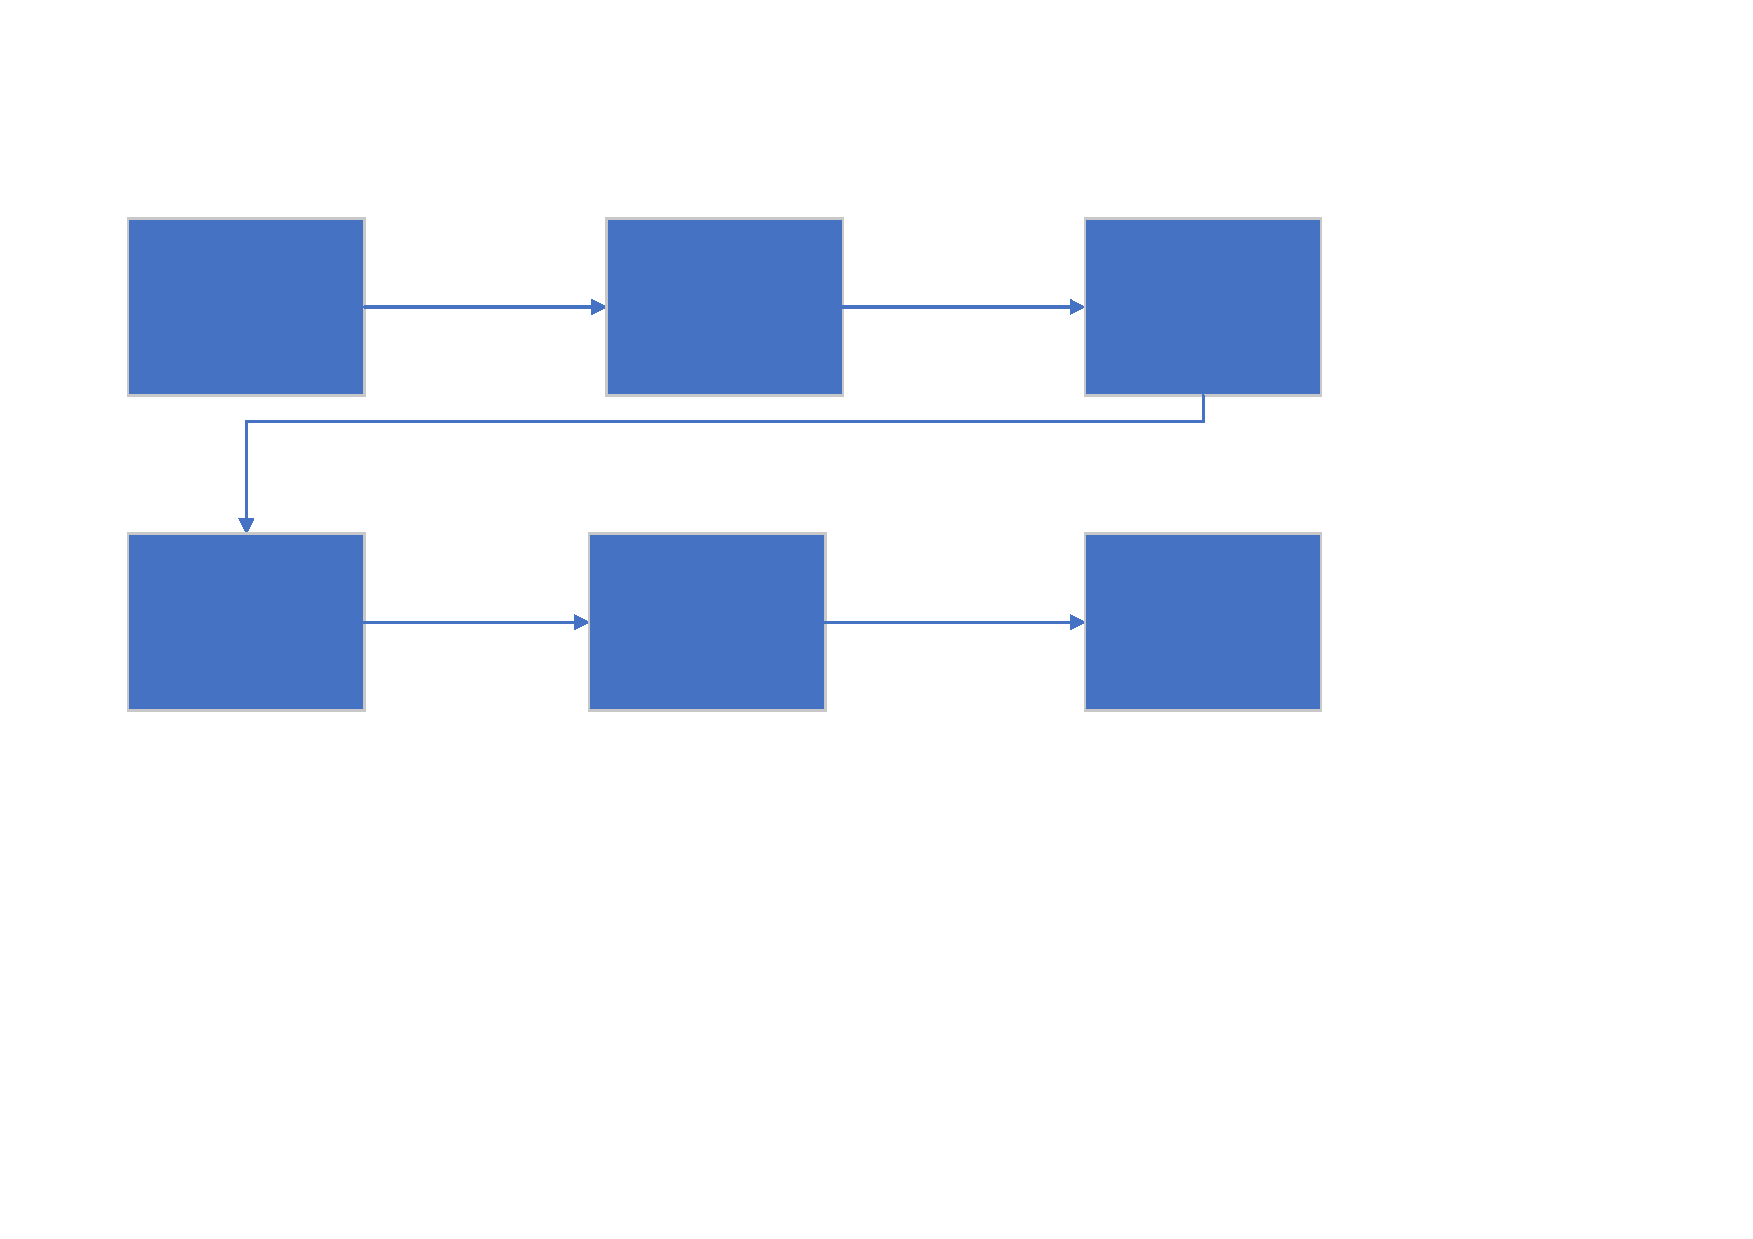
\includegraphics[scale=0.3]{diagram.pdf}

\section{Sources}


From Tabletop RPG to Interactive Storytelling: Definition of a Story 
Manager for Video Games – Guylain Delmas, Ronan Champagnat, Michel 
Augeraud

An Interactive Storytelling Model for Non-Player Characters on Electronic 
RPGs – Artur O. R. Franco, José G. R. Maia, Joaquim A. M. Neto, Fernando 
A. C. Gomes

Serious Storytelling: Narrative Considerations for Serious Games 
Researchers and Developers – Rudy McDaniel, Stephen M. Fiore, Denise 
Nicholson

\end{document}
